\documentclass[a4paper,12pt]{paper}

\usepackage{mycommands}

% Worked-example layout: boxed problem statement followed by a solution.
\newcounter{example}
\renewenvironment{example}[1]{%  % paper.cls already defines an example environment
  \refstepcounter{example}%
  \begin{mdframed}[linewidth=1pt,innertopmargin=6pt,innerbottommargin=6pt]%
  \noindent\textbf{Example \theexample: #1.}\ }{%
  \end{mdframed}}
\newenvironment{solution}{\par\noindent\textbf{Solution.}\ }{\par\medskip}

\title{Worked examples for Lecture 12: Finite elasticity}
\author{David Al-Attar \\ Michaelmas Term, \the\year}

\begin{document}

\maketitle

\noindent These examples accompany Lecture~12. They are intended as practice in the concrete
calculations that underlie the lecture, and are less demanding than the questions on the
problem sets. Numerical results were checked with the scripts in the \texttt{python}
directory.

%----------------------------------------------------------------------------------------
\begin{example}{Simple shear}
A body with referential density $\rho(\mathbf{x})$ undergoes the motion
\begin{equation*}
\bphi(\mathbf{x},t)=(x_{1}+\gamma t\,x_{2},\;x_{2},\;x_{3}),
\end{equation*}
where $\gamma$ is a constant shear rate, and the reference body is the position of the body at
$t=0$. (a) Compute the referential velocity, the deformation gradient and the Jacobian, and
show that the motion preserves volume. (b) Find the inverse motion $\bphi^{-1}(\cdot,t)$, and
hence the spatial density and the spatial velocity field, i.e.\ the velocity of whichever
particle occupies the spatial point $\mathbf{y}$ at time $t$. Compare these with their
referential counterparts. (c) Compute $\mathbf{C}=\mathbf{F}^{T}\mathbf{F}$, show that
$\delta\mathbf{x}\cdot\mathbf{C}\,\delta\mathbf{x}$ is the squared length of the image of a
small material line element $\delta\mathbf{x}$, and find the eigenvalues and eigenvectors of
$\mathbf{C}$. The square roots of the eigenvalues are the \emph{principal stretches}.
\end{example}

\begin{solution}
(a) Differentiating the motion with respect to time at fixed $\mathbf{x}$, and with respect to
$\mathbf{x}$ at fixed $t$, we obtain
\begin{equation}
\mathbf{v}(\mathbf{x},t)=(\gamma x_{2},0,0),\quad
\mathbf{F}(\mathbf{x},t)=\begin{pmatrix}1&\gamma t&0\\0&1&0\\0&0&1\end{pmatrix}.
\label{eq:1}
\end{equation}
The deformation gradient is upper triangular with unit diagonal, and so
\begin{equation}
J=\det\mathbf{F}=1
\label{eq:2}
\end{equation}
for all $\mathbf{x}$ and $t$. Applying the change of variables formula with $f=1$ to any
sub-body $U$, we find that the volume of $U_{t}$ equals that of $U$, so the motion is
\emph{isochoric}. Mass conservation, $\rho(\mathbf{x})=J\varrho[\bphi(\mathbf{x},t),t]$, then
gives $\varrho[\bphi(\mathbf{x},t),t]=\rho(\mathbf{x})$: each particle retains its initial
density.

(b) Setting $\mathbf{y}=\bphi(\mathbf{x},t)$ and solving for $\mathbf{x}$ gives the inverse
motion
\begin{equation}
\bphi^{-1}(\mathbf{y},t)=(y_{1}-\gamma t\,y_{2},\;y_{2},\;y_{3}),
\label{eq:3}
\end{equation}
which is well-defined for all $t$, as it must be since $J\neq0$. The spatial density is
therefore
\begin{equation}
\varrho(\mathbf{y},t)=\rho(y_{1}-\gamma t\,y_{2},y_{2},y_{3}).
\label{eq:4}
\end{equation}
Although $J=1$, the spatial density at a fixed point $\mathbf{y}$ is in general
time-dependent. For example, if $\rho(\mathbf{x})=\rho_{0}(1+\alpha x_{1})$, then
$\varrho(\mathbf{y},t)=\rho_{0}[1+\alpha(y_{1}-\gamma t\,y_{2})]$, because particles of
differing density are carried past the point $\mathbf{y}$ by the shear. Only for uniform
$\rho$ is $\varrho$ constant in time. For the velocity, substituting eq.~(\ref{eq:3}) into
eq.~(\ref{eq:1}) gives the spatial velocity field
\begin{equation}
\mathbf{v}[\bphi^{-1}(\mathbf{y},t),t]=(\gamma y_{2},0,0).
\label{eq:5}
\end{equation}
For this particular motion the spatial and referential velocity fields have the same functional
form, because the velocity depends only on $x_{2}$, and $x_{2}=y_{2}$ is unchanged by the
motion. Their meanings are nevertheless different: eq.~(\ref{eq:1}) gives the velocity of the
particle labelled $\mathbf{x}$, while eq.~(\ref{eq:5}) gives the velocity observed at the fixed
spatial point $\mathbf{y}$. Example~4 provides a case in which the two fields differ in form.

(c) From eq.~(\ref{eq:1}), and writing $a=\gamma t$ for brevity,
\begin{equation}
\mathbf{C}=\mathbf{F}^{T}\mathbf{F}=\begin{pmatrix}1&a&0\\a&1+a^{2}&0\\0&0&1\end{pmatrix}.
\label{eq:6}
\end{equation}
By the Taylor expansion of the motion, a small material line element $\delta\mathbf{x}$ at
$\mathbf{x}$ is mapped to $\mathbf{F}\,\delta\mathbf{x}$, whose squared length is
\begin{equation}
\|\mathbf{F}\,\delta\mathbf{x}\|^{2}=\delta\mathbf{x}\cdot\mathbf{F}^{T}\mathbf{F}\,\delta\mathbf{x}
=\delta\mathbf{x}\cdot\mathbf{C}\,\delta\mathbf{x}.
\label{eq:7}
\end{equation}
Hence $\mathbf{C}$ is symmetric and positive-definite, and a unit line element along an
eigenvector of $\mathbf{C}$ with eigenvalue $\lambda$ has its length multiplied by
$\sqrt{\lambda}$. The $x_{3}$-direction is an eigenvector with eigenvalue $1$. In the
$(x_{1},x_{2})$-plane the characteristic equation is
\begin{equation}
\lambda^{2}-(2+a^{2})\lambda+1=0,
\label{eq:8}
\end{equation}
with roots
\begin{equation}
\lambda_{\pm}=1+\tfrac{1}{2}a^{2}\pm a\sqrt{1+\tfrac{1}{4}a^{2}}.
\label{eq:9}
\end{equation}
The product of the roots is $\lambda_{+}\lambda_{-}=1=\det\mathbf{C}=J^{2}$, as it must be for
an isochoric motion. The principal stretches take the simple form
\begin{equation}
\sqrt{\lambda_{\pm}}=\sqrt{1+\tfrac{1}{4}a^{2}}\pm\tfrac{1}{2}a,
\label{eq:10}
\end{equation}
as may be verified by squaring the right-hand side. The eigenvector equation
$(1-\lambda)u_{1}+au_{2}=0$ gives $\mathbf{u}\propto(1,(\lambda-1)/a,0)$, and using
eqs.~(\ref{eq:9}) and (\ref{eq:10}) we have
$(\lambda_{\pm}-1)/a=\tfrac{1}{2}a\pm\sqrt{1+\tfrac{1}{4}a^{2}}=\pm\sqrt{\lambda_{\pm}}$, so
that
\begin{equation}
\mathbf{u}_{\pm}\propto(1,\pm\sqrt{\lambda_{\pm}},0).
\label{eq:11}
\end{equation}
These are orthogonal, since $\mathbf{u}_{+}\cdot\mathbf{u}_{-}=1-\sqrt{\lambda_{+}\lambda_{-}}=0$.
For small $a$ we have $\lambda_{\pm}=1\pm a+O(a^{2})$, principal stretches $1\pm\tfrac{1}{2}a$,
and eigenvectors tending to $(1,\pm1,0)/\sqrt{2}$: to first order, simple shear is an extension
along one diagonal of the $(x_{1},x_{2})$-plane and an equal contraction along the other, which
is the familiar statement of small-strain theory. For large $a$ the largest stretch is
approximately $a$, and its direction $(1,\sqrt{\lambda_{+}},0)$ tends towards the
$x_{2}$-axis, since material lines initially along $x_{2}$ are drawn out most strongly by the
shear.
\end{solution}

%----------------------------------------------------------------------------------------
\begin{example}{Polar decomposition by hand}
Consider the plane deformation gradient
\begin{equation*}
\mathbf{F}=\begin{pmatrix}2&1\\0&1\end{pmatrix},
\end{equation*}
the third direction being trivial ($F_{33}=1$, $F_{13}=F_{23}=F_{31}=F_{32}=0$). The polar
decomposition theorem of Lecture~13 states that $\mathbf{F}=\mathbf{R}\mathbf{U}=\mathbf{V}\mathbf{R}$
with $\mathbf{R}$ a rotation matrix and $\mathbf{U}$, $\mathbf{V}$ symmetric and
positive-definite. Compute $\mathbf{C}=\mathbf{F}^{T}\mathbf{F}$ and its eigenvalues and
eigenvectors; construct $\mathbf{U}=\sqrt{\mathbf{C}}$ from the eigen-decomposition; show that
$\mathbf{R}=\mathbf{F}\mathbf{U}^{-1}$ is a rotation and find its angle; compute
$\mathbf{V}=\mathbf{R}\mathbf{U}\mathbf{R}^{T}$; and describe the image of the unit circle.
\end{example}

\begin{solution}
Direct multiplication gives
\begin{equation}
\mathbf{C}=\mathbf{F}^{T}\mathbf{F}=\begin{pmatrix}2&0\\1&1\end{pmatrix}
\begin{pmatrix}2&1\\0&1\end{pmatrix}=\begin{pmatrix}4&2\\2&2\end{pmatrix},
\label{eq:12}
\end{equation}
with $\tr\,\mathbf{C}=6$ and $\det\mathbf{C}=4=(\det\mathbf{F})^{2}$. The characteristic
equation $\lambda^{2}-6\lambda+4=0$ has roots
\begin{equation}
\lambda_{\pm}=3\pm\sqrt{5},
\label{eq:13}
\end{equation}
and the eigenvector equation $(4-\lambda)u_{1}+2u_{2}=0$ gives $\mathbf{u}\propto(2,\lambda-4)$,
so that
\begin{equation}
\mathbf{u}_{\pm}\propto(2,\,-1\pm\sqrt{5}),\quad
\|\mathbf{u}_{\pm}\|^{2}=10\mp2\sqrt{5}.
\label{eq:14}
\end{equation}
These are orthogonal, as $4-(\sqrt{5}-1)(\sqrt{5}+1)=0$. The eigenvector $\mathbf{u}_{+}$ makes
an angle $\alpha=\arctan[(\sqrt{5}-1)/2]\approx31.7^{\circ}$ with the $x_{1}$-axis. The square
roots of the eigenvalues have the closed forms
\begin{equation}
\sqrt{\lambda_{\pm}}=\frac{\sqrt{5}\pm1}{\sqrt{2}},
\label{eq:15}
\end{equation}
since $(\sqrt{5}\pm1)^{2}/2=(6\pm2\sqrt{5})/2=3\pm\sqrt{5}$; these are the principal
stretches, with product $2=\det\mathbf{F}$.

Writing $\mathbf{q}_{\pm}=\mathbf{u}_{\pm}/\|\mathbf{u}_{\pm}\|$, the square root of $\mathbf{C}$
is
\begin{equation}
\mathbf{U}=\sqrt{\lambda_{+}}\,\mathbf{q}_{+}\mathbf{q}_{+}^{T}+\sqrt{\lambda_{-}}\,\mathbf{q}_{-}\mathbf{q}_{-}^{T}.
\label{eq:16}
\end{equation}
Using $1/(10-2\sqrt{5})=(5+\sqrt{5})/40$, the first projector is
\begin{equation}
\mathbf{q}_{+}\mathbf{q}_{+}^{T}=\frac{5+\sqrt{5}}{40}\begin{pmatrix}4&2\sqrt{5}-2\\2\sqrt{5}-2&6-2\sqrt{5}\end{pmatrix}
=\begin{pmatrix}\frac{5+\sqrt{5}}{10}&\frac{\sqrt{5}}{5}\\[4pt]\frac{\sqrt{5}}{5}&\frac{5-\sqrt{5}}{10}\end{pmatrix},
\label{eq:17}
\end{equation}
and $\mathbf{q}_{-}\mathbf{q}_{-}^{T}=\mathbf{1}-\mathbf{q}_{+}\mathbf{q}_{+}^{T}$. Substituting
into eq.~(\ref{eq:16}) with eq.~(\ref{eq:15}), the entries of $\mathbf{U}$ are
\begin{align}
U_{11}&=\frac{(\sqrt{5}+1)(5+\sqrt{5})+(\sqrt{5}-1)(5-\sqrt{5})}{10\sqrt{2}}=\frac{12\sqrt{5}}{10\sqrt{2}}=\frac{6}{\sqrt{10}},\nonumber\\
U_{22}&=\frac{(\sqrt{5}+1)(5-\sqrt{5})+(\sqrt{5}-1)(5+\sqrt{5})}{10\sqrt{2}}=\frac{8\sqrt{5}}{10\sqrt{2}}=\frac{4}{\sqrt{10}},\nonumber\\
U_{12}&=\frac{\sqrt{5}}{5}\left(\sqrt{\lambda_{+}}-\sqrt{\lambda_{-}}\right)=\frac{2}{\sqrt{10}}.
\label{eq:18}
\end{align}
Hence
\begin{equation}
\mathbf{U}=\frac{1}{\sqrt{10}}\begin{pmatrix}6&2\\2&4\end{pmatrix}
=\sqrt{\frac{2}{5}}\begin{pmatrix}3&1\\1&2\end{pmatrix},
\label{eq:19}
\end{equation}
and we check that $\mathbf{U}^{2}=\frac{2}{5}\begin{pmatrix}10&5\\5&5\end{pmatrix}=\mathbf{C}$,
$\tr\,\mathbf{U}=\sqrt{10}=\sqrt{\lambda_{+}}+\sqrt{\lambda_{-}}$ and
$\det\mathbf{U}=2=\det\mathbf{F}$. (In two dimensions there is a shortcut: the
Cayley--Hamilton theorem gives $\mathbf{U}^{2}-(\tr\,\mathbf{U})\mathbf{U}+(\det\mathbf{U})\mathbf{1}=\mathbf{0}$,
so $\mathbf{U}=(\mathbf{C}+\sqrt{\det\mathbf{C}}\,\mathbf{1})/\tr\,\mathbf{U}$ with
$(\tr\,\mathbf{U})^{2}=\tr\,\mathbf{C}+2\sqrt{\det\mathbf{C}}=10$, which reproduces
eq.~(\ref{eq:19}) immediately.)

Inverting the $2\times2$ matrix,
\begin{equation}
\mathbf{U}^{-1}=\frac{1}{\det\mathbf{U}}\begin{pmatrix}U_{22}&-U_{12}\\-U_{12}&U_{11}\end{pmatrix}
=\frac{1}{\sqrt{10}}\begin{pmatrix}2&-1\\-1&3\end{pmatrix},
\label{eq:20}
\end{equation}
and therefore
\begin{equation}
\mathbf{R}=\mathbf{F}\mathbf{U}^{-1}=\frac{1}{\sqrt{10}}\begin{pmatrix}2&1\\0&1\end{pmatrix}
\begin{pmatrix}2&-1\\-1&3\end{pmatrix}=\frac{1}{\sqrt{10}}\begin{pmatrix}3&1\\-1&3\end{pmatrix}.
\label{eq:21}
\end{equation}
The columns of $\mathbf{R}$ are orthonormal, so $\mathbf{R}^{T}\mathbf{R}=\mathbf{1}$, and
$\det\mathbf{R}=(9+1)/10=1$; hence $\mathbf{R}$ is a rotation. Comparing with
$\begin{pmatrix}\cos\theta&-\sin\theta\\\sin\theta&\cos\theta\end{pmatrix}$ we read off
$\cos\theta=3/\sqrt{10}$ and $\sin\theta=-1/\sqrt{10}$, so that
\begin{equation}
\tan\theta=-\tfrac{1}{3},\quad\theta\approx-18.4^{\circ},
\label{eq:22}
\end{equation}
a clockwise rotation. The left stretch is most easily found from
$\mathbf{V}=\mathbf{R}\mathbf{U}\mathbf{R}^{T}=\mathbf{F}\mathbf{R}^{T}$:
\begin{equation}
\mathbf{V}=\frac{1}{\sqrt{10}}\begin{pmatrix}2&1\\0&1\end{pmatrix}\begin{pmatrix}3&-1\\1&3\end{pmatrix}
=\frac{1}{\sqrt{10}}\begin{pmatrix}7&1\\1&3\end{pmatrix},
\label{eq:23}
\end{equation}
which is symmetric with $\tr\,\mathbf{V}=\sqrt{10}$ and $\det\mathbf{V}=2$, so it has the same
eigenvalues as $\mathbf{U}$, and $\mathbf{V}^{2}=\begin{pmatrix}5&1\\1&1\end{pmatrix}=\mathbf{F}\mathbf{F}^{T}$.
As a final check,
\begin{equation}
\mathbf{V}\mathbf{R}=\frac{1}{10}\begin{pmatrix}7&1\\1&3\end{pmatrix}\begin{pmatrix}3&1\\-1&3\end{pmatrix}
=\frac{1}{10}\begin{pmatrix}20&10\\0&10\end{pmatrix}=\mathbf{F},
\label{eq:24}
\end{equation}
and similarly $\mathbf{R}\mathbf{U}=\mathbf{F}$. The eigenvectors of $\mathbf{V}$ are those of
$\mathbf{F}\mathbf{F}^{T}$, namely $\mathbf{w}_{\pm}\propto(1,-2\pm\sqrt{5})$, and one verifies
that $\mathbf{R}\mathbf{u}_{+}\propto\mathbf{w}_{+}$: the eigenvectors of $\mathbf{V}$ are the
rotated eigenvectors of $\mathbf{U}$. Indeed $\mathbf{w}_{+}$ makes an angle
$\beta=\arctan(\sqrt{5}-2)\approx13.3^{\circ}=\alpha+\theta$ with the $x_{1}$-axis.

\begin{figure}[ht]
    \centering
    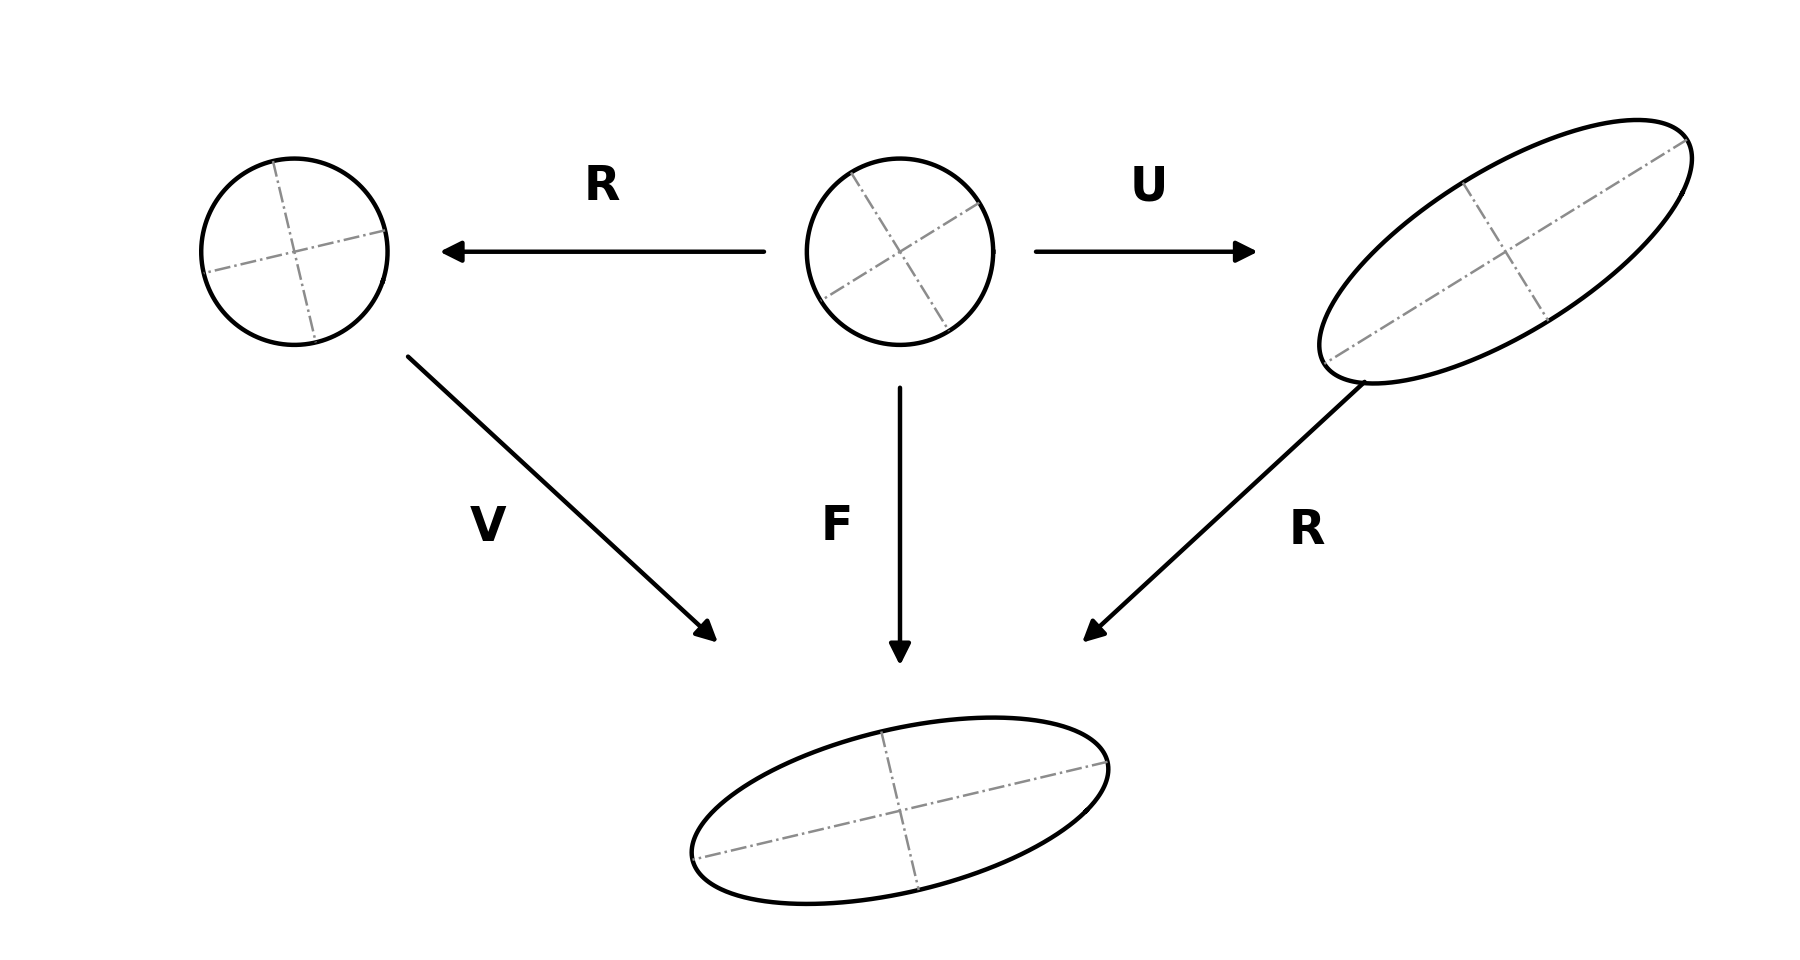
\includegraphics[width=0.7\textwidth]{figures_ex/ex1_polar.png}
    \caption{The polar decomposition of the deformation gradient of Example~2, drawn in
    the manner of the corresponding figure in Lecture~13. The unit circle (centre of
    the upper row) is stretched by $\mathbf{U}$ along its eigenvectors (dash-dotted lines, at
    $31.7^{\circ}$ and $121.7^{\circ}$) into an ellipse with semi-axes $2.29$ and $0.87$, and
    rotated by $\mathbf{R}$ through $-18.4^{\circ}$. Either order of operations produces the
    same final ellipse, whose axes lie along the eigenvectors of $\mathbf{V}$.}
    \label{fig:1}
\end{figure}

Geometrically (Fig.~\ref{fig:1}), $\mathbf{F}$ maps the unit circle to an ellipse with
semi-axes $\sqrt{\lambda_{\pm}}\approx2.29$ and $0.87$ along $\mathbf{w}_{\pm}$, whose area
$\pi\sqrt{\lambda_{+}\lambda_{-}}=2\pi$ is $J$ times that of the circle. The decomposition
$\mathbf{F}=\mathbf{R}\mathbf{U}$ realises this as a stretch along the fixed directions
$\mathbf{q}_{\pm}$ followed by the rotation, while $\mathbf{F}=\mathbf{V}\mathbf{R}$ rotates
first and then stretches along the co-rotated directions $\mathbf{w}_{\pm}=\mathbf{R}\mathbf{q}_{\pm}$.
Note that this matrix is the deformation gradient of the simple shear of Example~1 with
$\gamma t=1$, composed with a stretch by a factor of $2$ along $x_{1}$; neither ingredient
is a rotation, yet the deformation contains a rotation of $18.4^{\circ}$ that only the polar
decomposition makes visible.
\end{solution}

%----------------------------------------------------------------------------------------
\begin{example}{Rigid body motions}
Let $\bphi(\mathbf{x},t)=\mathbf{a}(t)+\mathbf{Q}(t)\mathbf{x}$, with $\mathbf{a}(t)$ a
translation and $\mathbf{Q}(t)$ a rotation matrix. (a) Show that $\mathbf{F}=\mathbf{Q}$,
$J=1$ and $\mathbf{C}=\mathbf{1}$. (b) Show that, if the origin of the reference body is
placed at its centre of mass, the kinetic energy is
$\tfrac{1}{2}M\|\dot{\mathbf{a}}\|^{2}$ plus a rotational term, and identify the latter.
(c) Show that any strain energy function satisfying material frame indifference has
$W(\mathbf{x},\mathbf{Q})=W(\mathbf{x},\mathbf{1})$, so that the potential energy is
unchanged by the motion. (d) Determine which of
$W_{1}=\tfrac{1}{2}\mu\,\tr(\mathbf{F}^{T}\mathbf{F}-\mathbf{1})$,
$W_{2}=\tfrac{1}{2}\mu\,\tr(\mathbf{F}-\mathbf{1})$ and
$W_{3}=\tfrac{1}{2}\mu\|\mathbf{F}-\mathbf{1}\|^{2}$, where $\|\mathbf{A}\|^{2}=A_{ij}A_{ij}$,
are frame indifferent, giving an explicit rotation $\mathbf{Q}$ for those that are not.
\end{example}

\begin{solution}
(a) Since $\varphi_{i}=a_{i}(t)+Q_{ij}(t)x_{j}$, we have
$F_{ij}=\partial\varphi_{i}/\partial x_{j}=Q_{ij}$. A rotation matrix satisfies
$\mathbf{Q}^{T}\mathbf{Q}=\mathbf{1}$ and $\det\mathbf{Q}=1$, so $J=1$ and
$\mathbf{C}=\mathbf{Q}^{T}\mathbf{Q}=\mathbf{1}$. By eq.~(\ref{eq:7}), no material line element
changes its length, which is what we mean by a rigid motion.

(b) The referential velocity is $\mathbf{v}=\dot{\mathbf{a}}+\dot{\mathbf{Q}}\mathbf{x}$.
Differentiating $\mathbf{Q}^{T}\mathbf{Q}=\mathbf{1}$ gives
$\dot{\mathbf{Q}}^{T}\mathbf{Q}+\mathbf{Q}^{T}\dot{\mathbf{Q}}=\mathbf{0}$, so the matrix
$\bm{\Omega}=\mathbf{Q}^{T}\dot{\mathbf{Q}}$ is antisymmetric and can be written
$\Omega_{ij}=-\epsilon_{ijk}\omega_{k}$ for some vector $\bm{\omega}(t)$, the angular velocity
referred to the reference body. Then $\bm{\Omega}\mathbf{x}=\bm{\omega}\times\mathbf{x}$ and
$\dot{\mathbf{Q}}\mathbf{x}=\mathbf{Q}(\bm{\omega}\times\mathbf{x})$, so that
\begin{equation}
\|\mathbf{v}\|^{2}=\|\dot{\mathbf{a}}\|^{2}+2\dot{\mathbf{a}}\cdot\mathbf{Q}(\bm{\omega}\times\mathbf{x})
+\|\bm{\omega}\times\mathbf{x}\|^{2},
\label{eq:25}
\end{equation}
where we used that $\mathbf{Q}$ preserves lengths. Integrating against $\rho$ over $M$, the
middle term contains $\int_{M}\rho\,\mathbf{x}\dd^{3}\mathbf{x}$, which vanishes when the
origin is at the centre of mass. Using
$\|\bm{\omega}\times\mathbf{x}\|^{2}=\|\bm{\omega}\|^{2}\|\mathbf{x}\|^{2}-(\bm{\omega}\cdot\mathbf{x})^{2}$,
the kinetic energy becomes
\begin{equation}
\mathcal{T}=\tfrac{1}{2}M\|\dot{\mathbf{a}}\|^{2}+\tfrac{1}{2}\omega_{i}I_{ij}\omega_{j},\quad
I_{ij}=\int_{M}\rho(\mathbf{x})\left(\|\mathbf{x}\|^{2}\delta_{ij}-x_{i}x_{j}\right)\dd^{3}\mathbf{x},
\label{eq:26}
\end{equation}
where $M=\int_{M}\rho\dd^{3}\mathbf{x}$ is the total mass and $I_{ij}$ is the inertia tensor
of the reference body, which is constant in time. This is the familiar decomposition of the
kinetic energy of a rigid body into translational and rotational parts, here obtained
directly from the referential formula of the lecture.

(c) Material frame indifference requires $W(\mathbf{x},\mathbf{Q}\mathbf{F})=W(\mathbf{x},\mathbf{F})$
for all deformation gradients and all rotations. Setting $\mathbf{F}=\mathbf{1}$ gives
$W(\mathbf{x},\mathbf{Q})=W(\mathbf{x},\mathbf{1})$, and hence for the rigid motion
\begin{equation}
\mathcal{V}(t)=\int_{M}W[\mathbf{x},\mathbf{Q}(t)]\dd^{3}\mathbf{x}=\int_{M}W(\mathbf{x},\mathbf{1})\dd^{3}\mathbf{x},
\label{eq:27}
\end{equation}
which is independent of time. The Lagrangian therefore reduces, up to a constant, to the
kinetic energy of eq.~(\ref{eq:26}), and Hamilton's principle would return the equations of
motion of a free rigid body.

(d) For $W_{1}$ we have
$W_{1}(\mathbf{Q}\mathbf{F})=\tfrac{1}{2}\mu\,\tr(\mathbf{F}^{T}\mathbf{Q}^{T}\mathbf{Q}\mathbf{F}-\mathbf{1})=W_{1}(\mathbf{F})$
for every rotation, so $W_{1}$ is frame indifferent; it depends on $\mathbf{F}$ only through
$\mathbf{C}$. For the other two it suffices to exhibit a single counterexample. Take the
rotation by $\pi/2$ about the $x_{3}$-axis,
\begin{equation}
\mathbf{Q}=\begin{pmatrix}0&-1&0\\1&0&0\\0&0&1\end{pmatrix},\quad\tr\,\mathbf{Q}=1,
\label{eq:28}
\end{equation}
and compare $\mathbf{F}=\mathbf{1}$ with $\mathbf{F}=\mathbf{Q}$. We find
$W_{2}(\mathbf{1})=0$ but $W_{2}(\mathbf{Q})=\tfrac{1}{2}\mu(1-3)=-\mu$, while
$W_{3}(\mathbf{1})=0$ but
\begin{equation}
W_{3}(\mathbf{Q})=\tfrac{1}{2}\mu(Q_{ij}-\delta_{ij})(Q_{ij}-\delta_{ij})
=\tfrac{1}{2}\mu(Q_{ij}Q_{ij}-2Q_{ii}+3)=\mu(3-\tr\,\mathbf{Q})=2\mu.
\label{eq:29}
\end{equation}
Neither $W_{2}$ nor $W_{3}$ is frame indifferent: both assign a change of potential energy to
a rigid rotation of the undeformed body. More generally, for a rotation through an angle
$\psi$ about any axis $\tr\,\mathbf{Q}=1+2\cos\psi$, so $W_{3}(\mathbf{Q})=2\mu(1-\cos\psi)$.
The function $W_{3}$ is what one obtains by naively treating the full displacement gradient,
rather than its symmetric part, as a measure of strain, and this calculation shows why the
linearised theory of the next lecture must be built from the symmetric strain tensor. Note
finally that frame indifference is necessary but not sufficient for a physically sensible
strain energy: $W_{1}$ passes the test, yet $\partial W_{1}/\partial F_{ij}=\mu F_{ij}$ does
not vanish at $\mathbf{F}=\mathbf{1}$, so a body with this strain energy is not stress-free
in its reference configuration.
\end{solution}

%----------------------------------------------------------------------------------------
\begin{example}{Uniform stretch of a cube}
Let the reference body $M$ be the unit cube $[0,1]^{3}$ with uniform referential density
$\rho$, and consider the motion
$\bphi(\mathbf{x},t)=(\lambda_{1}x_{1},\lambda_{2}x_{2},\lambda_{3}x_{3})$ with
$\lambda_{i}>0$. (a) Compute the mass, the volume of $M_{t}$ and the spatial density.
(b) Now let $\lambda_{i}=\lambda_{i}(t)$. Compute the kinetic energy from the referential
formula of the lecture, and again as an integral over $M_{t}$ of
$\tfrac{1}{2}\varrho\|\mathbf{v}\|^{2}$ with the spatial velocity field, and check that the
two agree.
\end{example}

\begin{solution}
(a) The deformation gradient is $\mathbf{F}=\mathrm{diag}(\lambda_{1},\lambda_{2},\lambda_{3})$
with $J=\lambda_{1}\lambda_{2}\lambda_{3}>0$. The instantaneous body is the box
$M_{t}=[0,\lambda_{1}]\times[0,\lambda_{2}]\times[0,\lambda_{3}]$, whose volume is
$\lambda_{1}\lambda_{2}\lambda_{3}=J$, in agreement with the change of variables formula
$\int_{M_{t}}\dd^{3}\mathbf{y}=\int_{M}J\dd^{3}\mathbf{x}$. The mass is
$\int_{M}\rho\dd^{3}\mathbf{x}=\rho$, and mass conservation gives the spatial density
\begin{equation}
\varrho(\mathbf{y},t)=\frac{\rho}{J}=\frac{\rho}{\lambda_{1}\lambda_{2}\lambda_{3}},
\label{eq:30}
\end{equation}
which is uniform, and satisfies $\int_{M_{t}}\varrho\dd^{3}\mathbf{y}=(\rho/J)J=\rho$ as it
must.

(b) The referential velocity is $v_{i}=\dot{\lambda}_{i}x_{i}$ (no sum on $i$), so the
kinetic energy is
\begin{equation}
\mathcal{T}=\frac{1}{2}\rho\int_{M}\sum_{i=1}^{3}\dot{\lambda}_{i}^{2}x_{i}^{2}\dd^{3}\mathbf{x}
=\frac{1}{2}\rho\sum_{i=1}^{3}\dot{\lambda}_{i}^{2}\int_{0}^{1}x_{i}^{2}\dd x_{i}
=\frac{\rho}{6}\left(\dot{\lambda}_{1}^{2}+\dot{\lambda}_{2}^{2}+\dot{\lambda}_{3}^{2}\right).
\label{eq:31}
\end{equation}
For the spatial calculation, the particle at $\mathbf{y}\in M_{t}$ is
$x_{i}=y_{i}/\lambda_{i}$, so the spatial velocity field is
\begin{equation}
v_{i}[\bphi^{-1}(\mathbf{y},t),t]=\frac{\dot{\lambda}_{i}}{\lambda_{i}}\,y_{i},
\label{eq:32}
\end{equation}
which, in contrast to Example~1, differs in form from the referential field. Using
eq.~(\ref{eq:30}) and $\int_{M_{t}}y_{1}^{2}\dd^{3}\mathbf{y}=\tfrac{1}{3}\lambda_{1}^{3}\lambda_{2}\lambda_{3}=\tfrac{1}{3}J\lambda_{1}^{2}$
(and similarly for $y_{2}$, $y_{3}$),
\begin{equation}
\frac{1}{2}\int_{M_{t}}\varrho\|\mathbf{v}\|^{2}\dd^{3}\mathbf{y}
=\frac{\rho}{2J}\sum_{i=1}^{3}\frac{\dot{\lambda}_{i}^{2}}{\lambda_{i}^{2}}\cdot\frac{J\lambda_{i}^{2}}{3}
=\frac{\rho}{6}\sum_{i=1}^{3}\dot{\lambda}_{i}^{2},
\label{eq:33}
\end{equation}
in agreement with eq.~(\ref{eq:31}). The two calculations are related by the change of
variables $\mathbf{y}=\bphi(\mathbf{x},t)$, under which $\varrho\dd^{3}\mathbf{y}=\rho\dd^{3}\mathbf{x}$;
the referential form is the more convenient because its domain of integration does not move.
\end{solution}

%----------------------------------------------------------------------------------------
\begin{example}{Hamilton's principle for an elastic rod}
A thin rod of unit cross-sectional area occupies $x\in[0,L]$ in its reference configuration
and has uniform referential density $\rho$. Its motion is a scalar function $\varphi(x,t)$,
with $v=\partial\varphi/\partial t$ and $F=\partial\varphi/\partial x$, and its strain energy
function is $W(F)=\tfrac{1}{2}E(F-1)^{2}$ with $E>0$ a constant. Starting from the action
with Lagrangian density $\tfrac{1}{2}\rho v^{2}-W(F)$, derive the equation of motion and the
natural boundary conditions at $x=0$ and $x=L$. Identify the first Piola--Kirchhoff stress.
Then linearise about the reference configuration by writing $\varphi=x+su$ and obtain the
wave equation and the wave speed.
\end{example}

\begin{solution}
The action is
\begin{equation}
\mathcal{S}(\varphi)=\int_{0}^{T}\int_{0}^{L}\left\{\frac{1}{2}\rho\left(\frac{\partial\varphi}{\partial t}\right)^{2}
-\frac{1}{2}E\left(\frac{\partial\varphi}{\partial x}-1\right)^{2}\right\}\dd x\dd t.
\label{eq:34}
\end{equation}
For a variation $\delta\varphi$ vanishing at $t=0$ and $t=T$, the first variation is
\begin{equation}
\delta\mathcal{S}=\int_{0}^{T}\int_{0}^{L}\left\{\rho\frac{\partial\varphi}{\partial t}\frac{\partial\delta\varphi}{\partial t}
-T\frac{\partial\delta\varphi}{\partial x}\right\}\dd x\dd t,\quad
T=\frac{\ddns W}{\ddns F}=E\left(\frac{\partial\varphi}{\partial x}-1\right).
\label{eq:35}
\end{equation}
Integrating the first term by parts in time, the boundary contribution vanishes by the
fixed end-point condition, while the second term is integrated by parts in $x$:
\begin{equation}
\delta\mathcal{S}=\int_{0}^{T}\int_{0}^{L}\left\{-\rho\frac{\partial^{2}\varphi}{\partial t^{2}}+\frac{\partial T}{\partial x}\right\}\delta\varphi\dd x\dd t
-\int_{0}^{T}\Big[T\,\delta\varphi\Big]_{x=0}^{x=L}\dd t.
\label{eq:36}
\end{equation}
For $\delta\mathcal{S}$ to vanish for all admissible variations, the volume and boundary
terms must vanish separately. Choosing $\delta\varphi$ supported in the interior gives the
Euler--Lagrange equation
\begin{equation}
\rho\frac{\partial^{2}\varphi}{\partial t^{2}}=\frac{\partial T}{\partial x}=E\frac{\partial^{2}\varphi}{\partial x^{2}},
\label{eq:37}
\end{equation}
and then choosing $\delta\varphi$ with arbitrary values at the ends gives the natural boundary
conditions $T(0,t)=T(L,t)=0$, i.e.\
\begin{equation}
\frac{\partial\varphi}{\partial x}=1\quad\mbox{at}\quad x=0\quad\mbox{and}\quad x=L.
\label{eq:38}
\end{equation}
Comparing with the lecture, $T=\partial W/\partial F$ is the one-dimensional first
Piola--Kirchhoff stress, eq.~(\ref{eq:37}) is $\rho\,\partial v/\partial t=\partial T/\partial x$,
and eq.~(\ref{eq:38}) is the traction-free condition $T\hat{n}=0$ with $\hat{n}=\pm1$ the
outward normal at the two ends. Physically, an element with $F>1$ is stretched and carries
the tension $E(F-1)$, an element with $F<1$ is compressed, and the free ends of the rod
carry no force. Had one end been held fixed instead, say $\varphi(0,t)=0$, the admissible
variations would satisfy $\delta\varphi(0,t)=0$, no boundary term would arise there, and the
condition at that end would be the prescribed (essential) one rather than a natural one.

Linearising, set $\varphi(x,t)=x+su(x,t)$ with $s$ small. Then $F=1+s\,\partial u/\partial x$,
$T=sE\,\partial u/\partial x$, and eq.~(\ref{eq:37}) becomes, after dividing by $s$,
\begin{equation}
\frac{\partial^{2}u}{\partial t^{2}}=c^{2}\frac{\partial^{2}u}{\partial x^{2}},\quad c=\sqrt{\frac{E}{\rho}},
\label{eq:39}
\end{equation}
with $\partial u/\partial x=0$ at the free ends. The normal modes are
$u=\cos(n\pi x/L)\cos(\omega_{n}t)$ with $\omega_{n}=n\pi c/L$. Because $W$ is quadratic in
$F$ the exact equation (\ref{eq:37}) was already linear, so here the linearisation is exact.
This cannot happen in three dimensions: a strain energy that is quadratic in $\mathbf{F}$ and
frame indifferent must be a linear function of $\mathbf{C}=\mathbf{F}^{T}\mathbf{F}$, and then
$\partial W/\partial F_{ij}$ is linear in $\mathbf{F}$ and non-zero at $\mathbf{F}=\mathbf{1}$
(as for $W_{1}$ in Example~3), so the reference configuration is not stress-free. The
linearisation carried out in Lecture~13 is therefore a genuine approximation.
\end{solution}

%----------------------------------------------------------------------------------------
\begin{example}{Traction as force per unit reference area}
Consider again the uniform stretch of Example~4, and suppose that the strain energy function
is $W(\mathbf{F})=\tfrac{1}{2}\kappa(J-1)^{2}$ with $\kappa>0$ constant and
$J=\det\mathbf{F}$. (a) Show that $\partial J/\partial F_{ij}=JF^{-1}_{ji}$, and hence compute
the first Piola--Kirchhoff stress. (b) Compute the traction $\mathbf{t}=\mathbf{T}\hat{\mathbf{n}}$
on the face $x_{1}=1$ of the reference cube, the total force acting on the image of this face,
and the corresponding force per unit \emph{current} area (the Cauchy traction). Show that the
two tractions differ by the factor $\lambda_{2}\lambda_{3}$.
\end{example}

\begin{solution}
(a) We first note that $W$ is frame indifferent, since
$\det(\mathbf{Q}\mathbf{F})=\det\mathbf{Q}\det\mathbf{F}=J$. To differentiate the determinant,
let $\delta\mathbf{F}$ be a small perturbation and write
$\mathbf{F}+\delta\mathbf{F}=\mathbf{F}(\mathbf{1}+\mathbf{F}^{-1}\delta\mathbf{F})$. For any
matrix $\mathbf{A}$, expanding the determinant shows that
$\det(\mathbf{1}+\mathbf{A})=1+\tr\,\mathbf{A}+O(\|\mathbf{A}\|^{2})$, because every term in
the expansion other than the product of the diagonal entries is at least quadratic in the
entries of $\mathbf{A}$. Hence
\begin{equation}
\det(\mathbf{F}+\delta\mathbf{F})=J\left[1+\tr(\mathbf{F}^{-1}\delta\mathbf{F})\right]+O(\|\delta\mathbf{F}\|^{2})
=J+JF^{-1}_{ji}\,\delta F_{ij}+O(\|\delta\mathbf{F}\|^{2}),
\label{eq:40}
\end{equation}
and comparing with $\delta J=(\partial J/\partial F_{ij})\delta F_{ij}$ we obtain
\begin{equation}
\frac{\partial J}{\partial F_{ij}}=JF^{-1}_{ji},
\label{eq:41}
\end{equation}
which is Jacobi's formula; note the transposed indices on the right-hand side. The chain rule
then gives the first Piola--Kirchhoff stress
\begin{equation}
T_{ij}=\frac{\partial W}{\partial F_{ij}}=\kappa(J-1)\frac{\partial J}{\partial F_{ij}}=\kappa(J-1)JF^{-1}_{ji},
\quad\mbox{i.e.}\quad\mathbf{T}=\kappa(J-1)J\mathbf{F}^{-T}.
\label{eq:42}
\end{equation}
For the uniform stretch $\mathbf{F}=\mathrm{diag}(\lambda_{1},\lambda_{2},\lambda_{3})$,
$J=\lambda_{1}\lambda_{2}\lambda_{3}$ and $\mathbf{F}^{-T}$ is diagonal with entries $\lambda_{i}^{-1}$,
so that
\begin{equation}
\mathbf{T}=\kappa(J-1)\,\mathrm{diag}(\lambda_{2}\lambda_{3},\;\lambda_{3}\lambda_{1},\;\lambda_{1}\lambda_{2}).
\label{eq:43}
\end{equation}

(b) On the face $x_{1}=1$ of the reference cube the outward unit normal is
$\hat{\mathbf{n}}=(1,0,0)$, and from eq.~(\ref{eq:43}) the traction is
\begin{equation}
\mathbf{t}=\mathbf{T}\hat{\mathbf{n}}=\kappa(J-1)\lambda_{2}\lambda_{3}\,(1,0,0).
\label{eq:44}
\end{equation}
This is the force per unit \emph{reference} area exerted on the body across the surface. The
face has unit area in the reference body, so the total force on its image is
$\kappa(J-1)\lambda_{2}\lambda_{3}$ in the $x_{1}$-direction. That image is the face
$y_{1}=\lambda_{1}$ of the box $M_{t}$, which has current area $\lambda_{2}\lambda_{3}$, so
the force per unit current area is
\begin{equation}
\mathbf{t}^{\mathrm{Cauchy}}=\frac{\kappa(J-1)\lambda_{2}\lambda_{3}}{\lambda_{2}\lambda_{3}}(1,0,0)=\kappa(J-1)(1,0,0),
\label{eq:45}
\end{equation}
and the two tractions differ by the factor $\lambda_{2}\lambda_{3}=J/\lambda_{1}$, the ratio
of current to reference area of the face. For $J>1$ the traction is directed outwards: an
outward pull must be applied to hold the body in a dilated state, and conversely a compressed
body ($J<1$) pushes back on whatever confines it.

The same argument applied to the other faces shows that the Cauchy traction on every face
is $\kappa(J-1)\hat{\mathbf{n}}_{t}$, with $\hat{\mathbf{n}}_{t}$ the current outward normal,
so the Cauchy stress is the isotropic tensor $\kappa(J-1)\mathbf{1}$: a body with this strain
energy behaves as a compressible fluid with pressure $-\kappa(J-1)$, and for small volume
changes $J-1\approx\nabla\cdot\mathbf{u}$ we recover the linear relation between pressure and
dilatation with bulk modulus $\kappa$. The general relation between the two stress tensors
is $\bm{\sigma}=J^{-1}\mathbf{T}\mathbf{F}^{T}$, which indeed reduces to $\kappa(J-1)\mathbf{1}$
for eq.~(\ref{eq:42}); the Piola--Kirchhoff and Cauchy stresses coincide only when
$\mathbf{F}=\mathbf{1}$, which is why their distinction can be ignored in linearised theories
about a stress-free reference state.
\end{solution}

\end{document}
